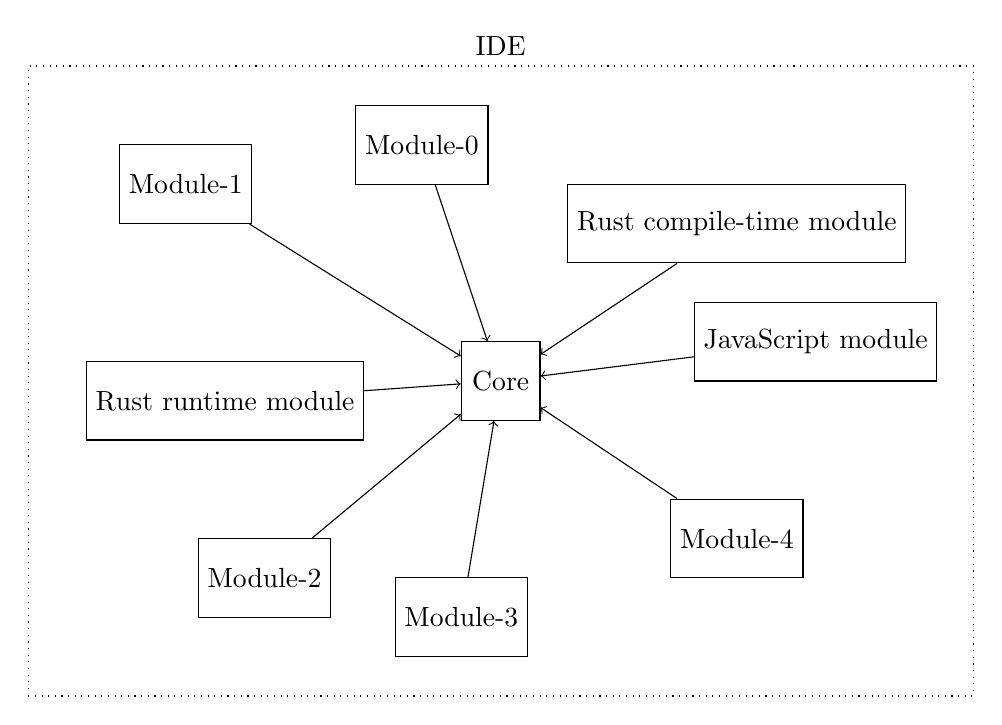
\begin{tikzpicture}
  \node (title) [] at (0, 4.25) {IDE};
  \node (x) [rectangle, draw, minimum height=8cm, minimum width=12cm, dotted] at (0, 0) {};
  % Nodes
  \node (core) [rectangle, draw, minimum height=1cm, minimum width=1cm] at (0, 0) {Core};
  \node (module-0) [rectangle, draw, minimum height=1cm, minimum width=1cm] at (4, 0.5) {JavaScript module};
  \node (module-1) [rectangle, draw, minimum height=1cm, minimum width=1cm] at (-3.5, -0.25) {Rust runtime module};
  \node (module-2) [rectangle, draw, minimum height=1cm, minimum width=1cm] at (3, 2) {Rust compile-time module};
  \node (module-3) [rectangle, draw, minimum height=1cm, minimum width=1cm] at (-1, 3) {Module-0};
  \node (module-4) [rectangle, draw, minimum height=1cm, minimum width=1cm] at (-4, 2.5) {Module-1};
  \node (module-5) [rectangle, draw, minimum height=1cm, minimum width=1cm] at (-3, -2.5) {Module-2};
  \node (module-6) [rectangle, draw, minimum height=1cm, minimum width=1cm] at (-0.5, -3) {Module-3};
  \node (module-7) [rectangle, draw, minimum height=1cm, minimum width=1cm] at (3, -2) {Module-4};
  % Arrow
  \draw[<-] (core) to node[midway, above] {} (module-0);
  \draw[<-] (core) to node[midway, above] {} (module-1);
  \draw[<-] (core) to node[midway, above] {} (module-2);
  \draw[<-] (core) to node[midway, above] {} (module-3);
  \draw[<-] (core) to node[midway, above] {} (module-4);
  \draw[<-] (core) to node[midway, above] {} (module-5);
  \draw[<-] (core) to node[midway, above] {} (module-6);
  \draw[<-] (core) to node[midway, above] {} (module-7);
  % Header
\end{tikzpicture}
